\scanpage{7}
\margin{\unsure{S|5}}

\figure{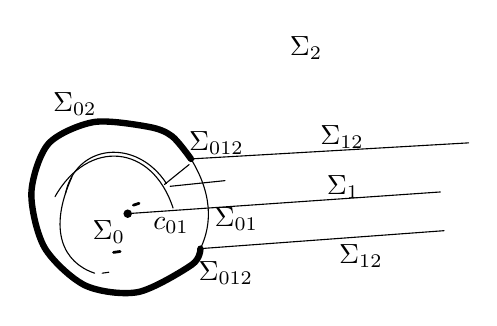
\begin{tikzpicture}[x=0.012cm,y=-0.012cm,line cap=round,line join=round]
\draw[line width=2.3pt] plot[smooth] coordinates {(436,274) (416,250) (391,240) (333,235) (285,258) (267,310) (281,368) (324,408) (380,415) (437,386) (446,369)};
\draw (436,274) .. controls (458,310) and (459,342) .. (446,369);
\draw (303,311) .. controls (314,258) and (378,251) .. (410,300);
\draw (292,314) .. controls (327,252) and (395,258) .. (417,326);
\draw (310,293) .. controls (284,350) and (301,384) .. (334,395);
\draw (342,395)--(349,394);
\draw (414,303)--(472,297) (408,301)--(434,280);
\draw (436,274)--(730,257) (368,332)--(700,309) (446,369)--(704,350);
\draw[line width=1pt] (375,323)--(381,321) (354,373)--(361,372);
\fill (369,332) circle (4.5);
\node at (558,157) {$\Sigma_2$};\node at (313,216) {$\Sigma_{02}$};
\node at (463,257) {$\Sigma_{012}$};\node at (596,251) {$\Sigma_{12}$};
\node at (349,351) {$\Sigma_0$};\node at (415,345) {$c_{01}$};
\node at (484,338) {$\Sigma_{01}$};\node at (597,304) {$\Sigma_1$};
\node at (473,395) {$\Sigma_{012}$};\node at (616,377) {$\Sigma_{12}$};
\end{tikzpicture}}

\margin{$\unsure{\supset d'}$}

\figure{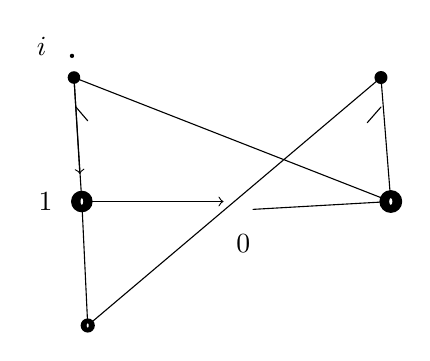
\begin{tikzpicture}[x=0.025cm,y=-0.025cm,line cap=round,line join=round]
\draw (1212,195)--(1373,258)--(1368,195)--(1219,321)--(1216,258);
\draw (1212,195)--(1216,258);
\draw[->] (1212,195)--(1215,244);
\draw[->] (1216,258)--(1288,258);
\draw (1303,262)--(1373,258);
\draw (1213,210)--(1219,217) (1368,210)--(1361,218);
\fill (1212,195) circle (3.2);
\fill (1216,258) circle (5.5);
\fill (1219,321) circle (3.6);
\fill (1368,195) circle (3.3);
\fill (1373,258) circle (5.8);
\fill (1211,184) circle (1.1);
\fill[white] (1216,258) ellipse (0.65 and 1.7);
\fill[white] (1219,321) ellipse (0.5 and 1.1);
\fill[white] (1373,258) ellipse (0.8 and 1.7);
\node[left] at (1203,179) {$\unsure{i}$};
\node[left] at (1206,258) {$1$};\node[below] at (1298,270) {$0$};
\end{tikzpicture}}

$\Sigma_{i_0i_1\ldots i_n}$\qquad\deleted{\unsure{covariant}} foncteur contravariant
par rapport aux drapeaux
variables $(i_0,\unsure{{:}\ldots|i_1\ldots},i_n)$

\[
\Sigma_i=X_i'=X_i\setminus\left(X_i\cap\bigcup_{k<i}\mathop{\overset{\unsure{\bullet|\deleted{\circ}}}{\mathrm{T}}\mathrm{ub}}\nolimits^{\circ}(X_k,X_i)\right)
\]

\[
\Sigma_{(i,j)}=\deleted{\unsure{\partial}}\operatorname{Tub}^{\bullet}\left(X_i',X_j\deleted{\unsure{\varnothing}}\setminus\bigcup_{\substack{\deleted{\unsure{k<j}}\quad\deleted{\unsure{i<k|j<k}}\\\deleted{\unsure{k\ne i}}\\\inserted{i<k<j}}}\operatorname{Tub}(X_k,X_j)\right)\hookrightarrow X_j'=\Sigma_j
\]

\[i<k<j\]

\margin{\diagram{\begin{tikzcd}
\Sigma_\delta\arrow[r,hook]\arrow[d]&\Sigma_{\delta'}\arrow[d]\\
\Sigma_d\arrow[r,hook]&\Sigma_{d'}
\end{tikzcd}}
\diagram{\[\begin{array}{ccc}d&\supset&d'\\&&\cap\\\unsure{\delta|d}&&\delta'\end{array}\]}
cofinaux
\diagram{\begin{tikzcd}\bullet\arrow[d]\\d'\end{tikzcd}}}

\deleted{$\Sigma_{i,j}=T.$}

\diagram{\begin{tikzcd}[column sep=small,row sep=large]
&\mathcal V_{i,j}\arrow[d]&{}=\mathcal V(X_i^*,X_j)\setminus\displaystyle\bigcup_{i\leq k<j}\mathcal V(\unsure{X_i^*|X_i'},X_j)\cap X_k\arrow[r,hook]&X_j^*\\
X&X_i^*&&
\end{tikzcd}}

\noindent $\mathcal V_{ijk}$\par

\diagram{\begin{tikzcd}[row sep=large,column sep=large,execute at end picture={\draw (branchend) ++(0.10,0.13)--(branchend)--++(0.16,-0.03);}]
\mathcal V_{ijk}\arrow[r]\arrow[d]&\mathcal V_{jk}\arrow[d]\arrow[r,hook,no head]&X_k^*\arrow[d,""{name=branch,coordinate,pos=.55}]\\
\mathcal V_{ij}\arrow[r,hook]\arrow[d]&\mathcal V(X_j^*,X_k)\arrow[r,phantom,"\deleted{\xrightarrow{\unsure{\sim}}}" description]&\deleted{X_k}\\
X_i^*&&
\arrow[from=branch,to=2-2,dashed,no head,to path={(\tikztostart)--++(-1.5,-0.45) coordinate (branchend)\tikztonodes},"\unsure{\sim|r}"']
\end{tikzcd}}

\margin{$\lambda_i'\unsure{T'|T^i}=\lambda''T''$\qquad
$a\leq\operatorname{Inf}(\lambda',\lambda_i')$}

\margin{\uline{6}}
